% 第3章
\chapter{実験環境}
 本章では,本研究で使用する歩行パターン生成器の説明及び実験環境やパラメータについて述べる.
本章では,本研究で行う実験に用いる実験環境や歩行パターン生成器について述べる.

\section{実験装置}
実験装置を表\ref{tab:Experimental Setup}に示す.また,本研究で使用する歩行パターン生成器は図のものである.はC++言語で実装されているMPCによる歩行パターン生成器である.表に示すライブラリ群を利用する.
\begin{table}[H]
  \centering
  \caption{Experimental Setup}
  \label{tab:Experimental Setup}
  \begin{tabular}{|l|l|}
      \hline \hline
       Device    & MacBook Air \\ \hline
       CPU       & Intel® Core™ i5-5250U CPU @ 1.60GHz × 4 \\ \hline
       RAM       & 7.7 GiB \\ \hline
       OS        & Ubuntu 20.04.6 LTS \\ \hline
  \end{tabular}
\end{table}

\begin{table}[H]
  \centering
  \caption{Libraries}
  \label{tab:Libraries}
  \begin{tabular}{|c|c|}
       \hline \hline
       QP solver                & osqp                  \\ \hline
       C++ binding of osqp      & osqp-eigen            \\ \hline
       Linear algebra library   & eigen-3.4.0           \\ \hline
  \end{tabular}
\end{table}

\begin{figure}[H]
  \centering
 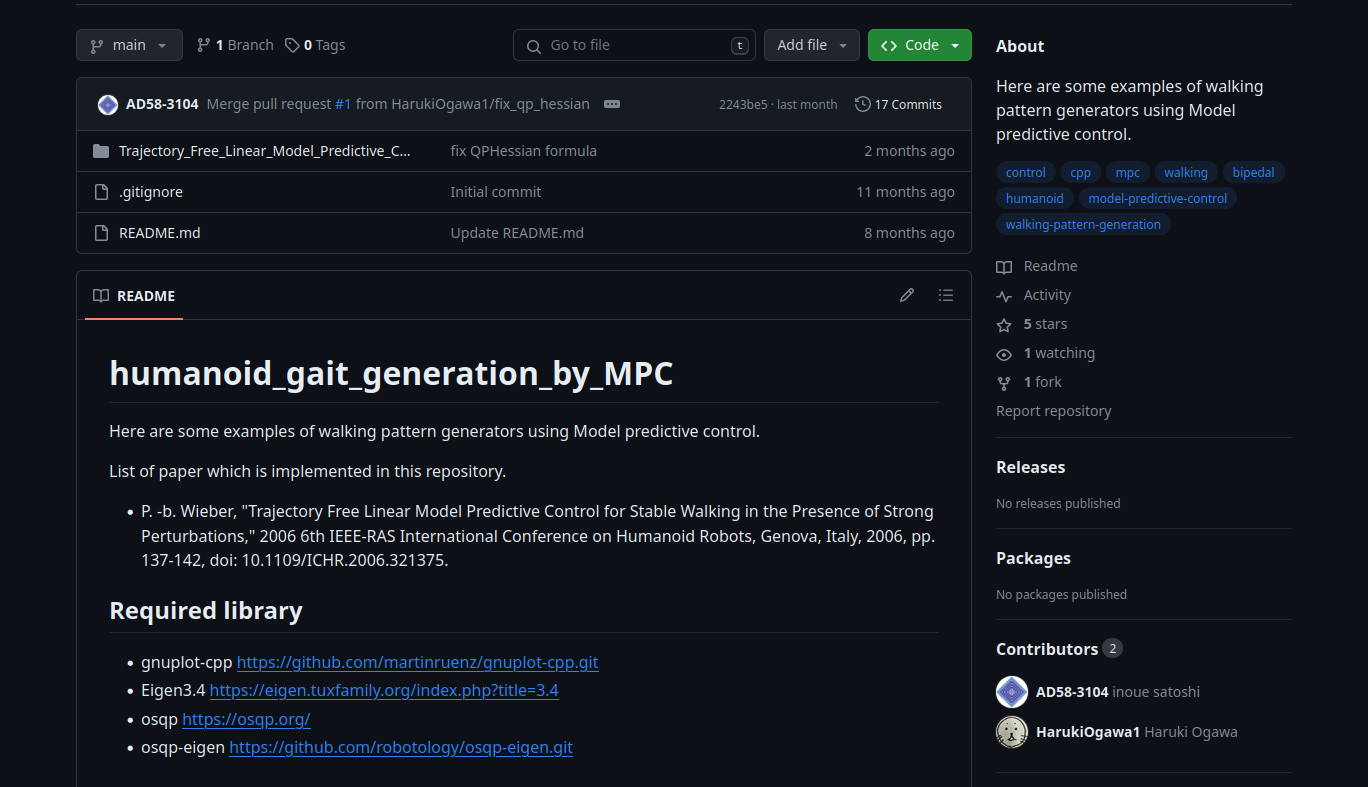
\includegraphics[keepaspectratio, scale=0.3]
      {images/github.png}
 \caption{GitHub page of publication}
 \label{Fig:GitHub page of publication}
\end{figure}


\section{本研究の歩行パターン生成器のパラメータ}
ここでは,4章に示す歩行パターンを生成可能なパラメータについて解説する.


\begin{table}[H]
  \centering
  \caption{Libraries used for implementation}
  \label{Libraries used for implementation}
  \begin{tabular}{|c|r|}
       \hline \hline
       Control Horizon                                          & 1.5{[}s{]}                      \\ \hline
       Unit time                                                & 10{[}s{]}                       \\ \hline
       Q / R                                                    & 1000000.0                        \\ \hline
       Height of CoM                                            & 0.6{[}m{]}                      \\ \hline
       Step width                                               & 0.15{[}m{]}                     \\ \hline
       start\_with\_this\_step                                  & 0.8{[}s{]}                      \\ \hline
       cycle\_step                                              & 0.4{[}s{]}                      \\ \hline
       double\_support\_step                                    & 0.1{[}s{]}                      \\ \hline \hline
       Upper bound of difference between ref and current output & 0.02{[}m{]}                     \\ \hline
       Lower bound of difference between ref and current output & -0.02{[}m{]}                    \\ \hline
       Upper bound of input                                     & 100{[}m/s\textsuperscript{3}{]} \\ \hline
       Lower bound of input                                     & 100{[}m/s\textsuperscript{3}{]} \\ \hline
  \end{tabular}
\end{table}

\begin{figure}[H]
  \centering
 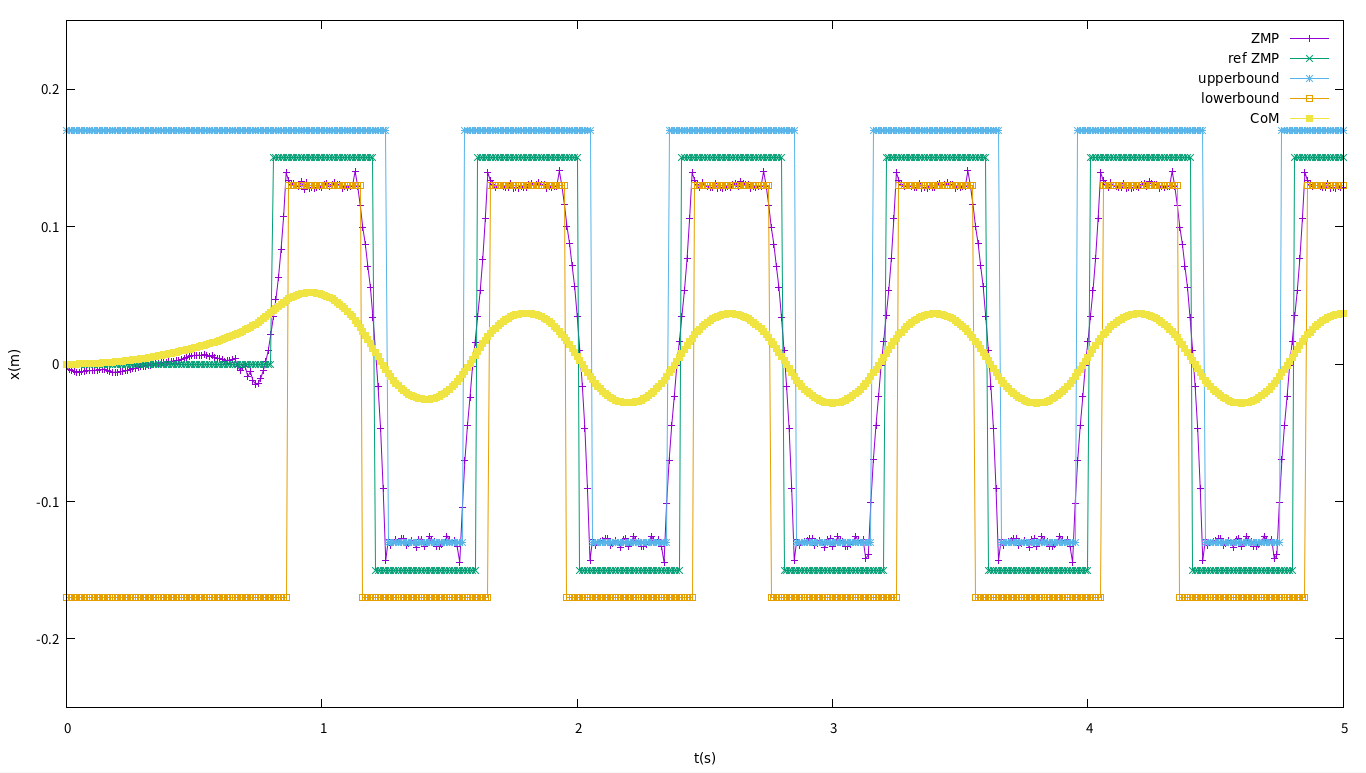
\includegraphics[keepaspectratio, scale=0.3]
      {images/mpc_sample.png}
 \caption{例になる歩行パターン}
 \label{Fig:例になる歩行パターン}
\end{figure}


\newpage